\chapter{工具原型设计}
本章节描述了整个工具原型的功能需求和主要处理步骤的设计。论文所述工具原型的主要功能是为C语言程序
生成一个保留了日志记录信息的有穷自动机,然后使用这样的自动机来分析C语言程序运行时刻产生的日志记录,获取该C语言程序的运行时刻信息,支持对该类程序的排错和维护。
主要子功能包括从 C语言程序 生成抽象语法树,从语法树生成不确定的有穷自动机,获取NFA中调用日志记录函数的信息并生成确定的有穷自动机(DFA),
以及使用这类有穷自动机来分析日志记录并获得C语言程序运行时刻的信息。

\section{工具原型的功能和主要模块设计}
本工具原型主要有两大功能,即根据输入的C语言程序生成能够反映其日志记录过程的确定有穷状态自动机的功能,以及使用该有穷自动机对
C语言程序在运行时产生的日志记录进行分析以获得其运行时信息的功能。

第一个功能分成如图\ref{fig:系统流程图}所示的主要步骤:
\begin{enumerate}
	\item 使用Clang库扫描C语言程序,生成该程序对应的抽象语法树Clang-AST;
    \item 通过遍历AST,处理C语言程序中的各个函数定义,并对函数体中的语句进行递归处理,生成基本的不确定有穷自动机NFA;
    \item 对C语言程序中各个函数对应的NFA进行处理,包括消除掉无关的信息,处理函数调用,并保留日志记录函数调用的信息,生成有关日志函数的NFA;
    \item 使用子集构造法,将此NFA转换成为确定的有穷状态自动机DFA。
\end{enumerate}

根据上面的处理过程,本工具原型的主要模块主要包括:Clang扫描模块,NFA生成模块,NFA到DFA的转换模块,以及日志序列扫描分析模块。

\textbf{Clang扫描模块}的过程比较简单,它直接调用Clang的接口,将 C语言 源代码转化为抽象语法树 (AST),

在生成 AST 后,\textbf{NFA生成模块}从抽象语法树的根节点开始,遍历抽象语法树的所有节点,对其中的每个对应于C函数定义的AST节点进行处理,生成对应的 NFA。
每个NFA使用Automaton类的对象表示。为了使得这个模块能够具有更好的扩展性,将来可能用于其它目的的程序分析工具,这个对象中还记录了相应抽象语法树节点的信息、
对于这个初始NFA,\textbf{NFA生成模块}将进一步处理,过滤掉针对日志记录分析无用的转换标签,仅保留日志记录函数调用信息。
经过处理后,原来仅仅保护无用标签的边将被视作空边处理。

\textbf{NFA到DFA的转换模块}使用子集构造法,将带有日志记录的NFA转化为确定的有穷自动机DFA。该模块首先实现了对于NFA中的状态,返回其epsilon闭包(通过空边换可以到达的所有状态的集合)的函数,接着调用返回epsilon闭包的函数,在算法中“并行地模拟”NFA在遇到一个给定输入串
时可能执行的所有动作,最终构造得到的DFA的每个状态和NFA的状态子集对应。\\


第二个功能,\textbf{日志序列扫描分析模块}将待处理的日志序列作为上面构造的DFA的输入,通过追踪记录DFA识别过程中的状态转移序列来分析日志序列,获取C语言程序的运行状态信息。在此过程中,模块能够根据DFA的规则解析日志序列,验证其是否符合预期的模式。对于合法掉日志序列,该模块将返回一个包含经过的DFA状态的列表。
通过这些列表,工具原型可以分析出C语言程序运行时刻的行为和相关信息。


\begin{figure}[htbp]
	\centering
	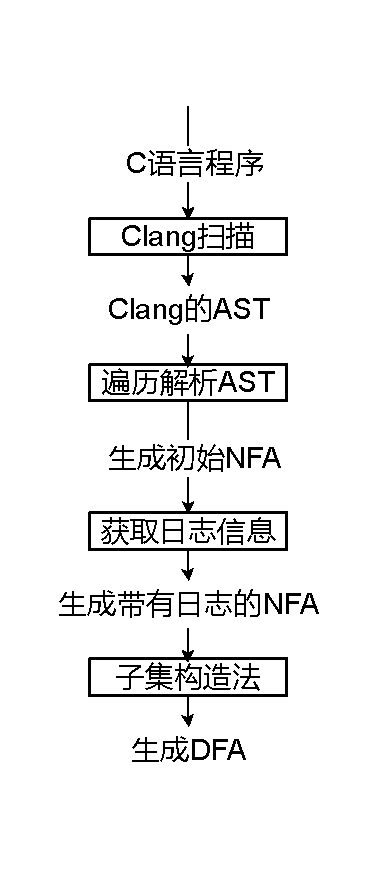
\includegraphics[width=0.25\textwidth]{pictures/系统流程图.pdf}
	\caption{系统流程图}
	\label{fig:系统流程图}
\end{figure}

\section{有穷自动机作为日志序列分析的基础}
一个系统在运行时会产生一系列的日志记录。这些日志在某种程度上记录了程序运行的历史,它也是系统维护和排错的重要依据。
程序员需要从日志记录中分析出尽可能多的系统运行信息,以提高维护和排错的效率。

因为效率的原因,系统通常只会记录关键事件的日志信息,导致从日志序列分析出系统运行信息变得相对困难。结合系统代码的信息,可以帮助人们从日志中分析得到更多的系统运行信息。
因此,本文使用有穷自动机对系统的源代码进行抽象描述,使之一方面能够反映源代码中的控制流信息,另一方面又能够高效处理日志记录序列。
首先对系统的源程序进行分析并生成有穷自动机,然后使用这个自动机高效地扫描输入的日志序列,
并根据扫描过程中经过的自动机的状态序列来获得更多的信息运行时刻信息。

源代码的控制流信息可以用有穷自动机来抽象地描述。
例如,对于程序中的每一条简单语句,可以直接使用一个简单的自动机来描述,形式为“状态1 -> 状态2”,其中状态1表示该语句的起始位置,状态2表示该语句的结束位置,而在转换的边上可以标注上这条语句的相关信息。而对于复杂语句,工具原型可以递归地为它的每个子语句生成相应的自动机。然后根据复杂语句的控制流结构,将子语句对应的自动机组合成为该复杂语句对应的自动机。诸如break、continue、return这样的控制流跳转语句,可以转换成为自动机状态之间的转换。
虽然这样构造的自动机忽略了很多源代码中的信息,但是它仍然能够在一定程度上反应出程序执行的控制流信息。

因为本文的目标是使用自动机来进行日志记录分析,因此源代码中对日志记录函数的调用被设置为自动机中相应转换的标号,而其它和日志记录无关的语句、表达式等被转换成为自动机中的$\epsilon$-转换。这个过程可以得到一个包含了程序的日志记录信息的不确定的有穷自动机。为了提高分析效率,本文将这个不确定有穷自动机转换成为确定的有穷自动机,并使用确定的有穷自动机高效地扫描和分析日志序列。
这样的处理使得自动机抽象地描述了程序的实际运行和日志记录情况。当自动机运行时,它会依据输入的条日志序列选择相应的边进行状态转换。
换句话说,这样的有穷自动机描述了日志生成的可能顺序,从而在一定程度上反映了程序的运行状态。

例如,如果系统的源程序有一条对日志记录函数的调用log("inside funcA"),表示程序执行到函数A内部。那么对应的自动机片段如图\ref{fig:日志函数对应的自动机片段}所示。

\begin{figure}[htbp]
	\centering
	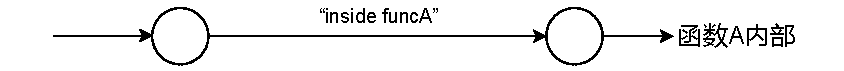
\includegraphics[width=1\textwidth]{pictures/函数调用示例.pdf}
	\caption{日志函数对应的自动机片段}
	\label{fig:日志函数对应的自动机片段}
\end{figure}
当程序执行中经过此语句时会向日志记录文件中插入一条"inside funcA"的日志记录。相应的,如果自动机分析日志记录文件中的日志序列时读入了"inside funcA", 它就能够判断系统程序在当时执行了语句log("inside fucA"),也就能判断出当时系统程序正在执行函数funcA。结合整个日志序列中的其它日志记录,就可以更加精确地分析出系统运行的信息。


\section{数据结构设计}
工具原型中主要有两类数据结构:一类是记录自动机信息的数据结构 Automaton,另一类是管理源程序的所有有穷自动机的数据结构 AutomatonManager。


\subsubsection{记录自动机信息的数据结构}
\begin{figure}[htbp]
	\centering
	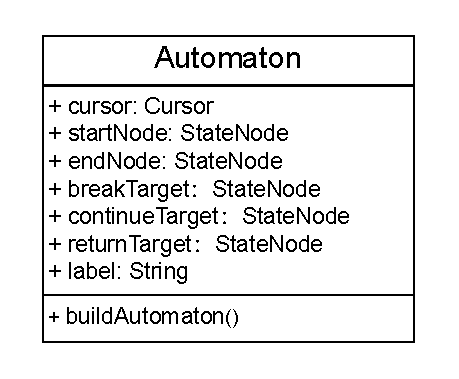
\includegraphics[width=0.5\textwidth]{pictures/Automaton的数据结构.pdf}
	\caption{Automaton的数据结构}
	\label{fig:Automaton的数据结构}
\end{figure}


Automaton类的对象记录了AST结点对应的自动机入口和出口和其他自动机的相关信息。
它的成员变量和方法如图\ref{fig:Automaton的数据结构}所示。

Automaton类的对象存有代表start和end的StateNode。StateNode类的对象代表了自动机的状态,它存有一个唯一的id,用于区分不同的状态。
其中Cursor类的对象cursor指向了相应的AST树结点,可以简单的将其看作对AST节点的“引用”。
此外,Automaton类的对象中还存有break语句,continue语句和return语句的跳转目标,它们以stateNode的形式表示,当下一层次的语句中存在
跳转语句时,便可将跳转语句的出口连接到相应的跳转目标上。
最后Automaton类的对象以字符串的形式储存了一个标签,用于表示边“startNode-->endNode”上的标签。

Automaton类中实现了buildAutomaton方法,当调用此方法时,如果对象为复杂语句,
会为当前语句的下一层次的语句生成相应的自动机片段,形成代表复杂语句的自动机层次结构,并将相关信息记录到Automaton类的对象;如果对象为简单语句,则不做处理。

对于简单语句,工具原型生成一个Automaton类的对象,它具有startNode和endNode两个state节点,并且有一条边从startNode连到endNode。

对于复杂语句,工具原型将生成一个Automaton类的对象,然后调用Automaton的方buildAutomaton,
这将为该语句的下一层次的语句也生成Automaton类的对象,从而递归地生成该复杂语句的自动机结构。

对于日志函数,工具原型同样地生成一个Automaton类的对象,其中边上的标签为日志函数“log”的输入参数。




\subsubsection{管理所有有穷自动机的数据结构}
\begin{figure}[htbp]
	\centering
	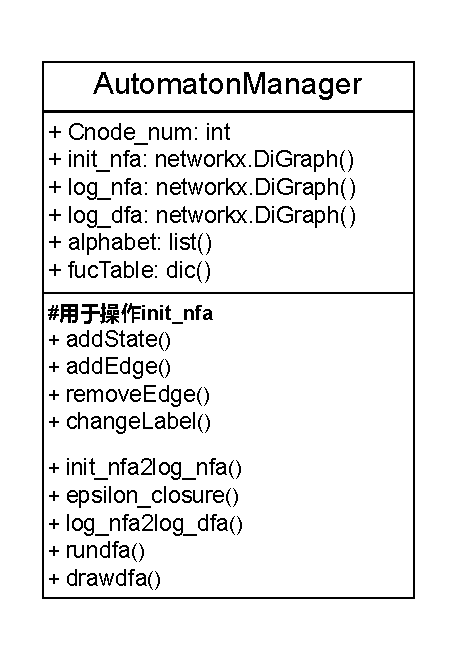
\includegraphics[width=0.5\textwidth]{pictures/AutomatonManager的数据结构.pdf}
	\caption{AutomatonManager的数据结构}
	\label{fig:AutomatonManager的数据结构}
\end{figure}
如图\ref{fig:AutomatonManager的数据结构},AutomatonManager类的对象以有向图的形式维护了所有生成的Automaton类的对象的连接信息,并实现了不同类型的图之间的转换方法。

AutomatonManager类的对象管理了所有生成的自动机,并将它们整合成一个代表C语言程序的自动机,其底层的数据结构是NetworkX库\cite{networkx}中的DiGraph类,它提供了一个易于维护的有向图结构,有向图中的节点代表自动机的状态,连边代表自动机的转移,边上的标签代表转移的输入字符。

AutomatonManager类的对象中有三个DiGraph类的对象:init\_nfa, log\_nfa和 log\_dfa,代表了工具原型运行到不同阶段时,代表C语言程序的不同类型的自动机。
\begin{itemize}
    \item  init\_nfa代表从AST树转换得到的非确定的有穷自动机。AutomatonManager类提供了修改该NFA的方法,可用于对自动机的图结构进行操作。如 addState() 可向init\_nfa中添加代表状态节点;addEdge(),removeEdge()可用于向init\_nfa中添加或者移除边;changeLabel()可用于添加或修改边上的标签。
自动机边的标签。
    \item  log\_nfa是在init\_nfa的基础上,删除掉无关信息,仅保留日志记录作为输入字符的非确定的有穷自动机。
    \item  log\_dfa则是根据 log\_nfa,利用子集构造法生成相应的确定的有穷自动机,其中一个DFA状态代表了一个NFA的状态集合。
\end{itemize}

除了维护自动机的图结构,AutomatonManager类还存有一个列表类型(list)的alphabet对象,用于储存所有日志函数的参数,作为自动机的合法输入字符集合。

最后,在处理 AST 中的函数调用节点时,AutomatonManager 类维护一个字典类型(dict)的 fucTable,用于将函数名映射到相应的 Automaton 对象。每当工具原型遇到函数调用节点时,会在 fucTable 中查找与该函数名对应的 Automaton 对象,并将该对象所记录的自动机连接到函数调用的位置。这种映射机制确保了函数调用的行为能够被精确地解析和执行。\\

AutomatonManager类还实现了不同自动机的图结构的转换方法,以及通过工具原型生成的DFA解析日志记录文件的方法。

首先,AutomatonManager类中实现了根据init\_nfa,生成带有日志函数的非确定有穷自动机  log\_nfa的方法:init\_nfa2 log\_nfa。它去除init\_nfa的有向图结构中的所有与日志函数无关的标签,使得所有日志函数的参数成为  log\_nfa 中的输入字符集合。

接着,该类实现了从非确定有穷自动机到确定的有穷自动机的转换方法  log\_nfa2 log\_dfa。它根据子集构造法,将  log\_nfa 进行转换,并存在 log\_dfa中。

最后,该类实现了一个根据已有的确定有穷自动机来解析日志的方法 rundfa。它以日志记录文件作为为输入序列,运行得到的DFA,并根据运行结果给出相应的分析:如日志合法性,C语言程序发生错误前的运行过程等。
\section{本章小结}
本章首先介绍了工具原型的功能,包括利用Clang生成抽象语法树,
根据AST生成NFA和DFA,以及使用DFA进行日志解析等功能。

然后描述了工具原型的模块设计,并对每个模块进行了解释。

接下来,文章围绕程序与自动机的对应关系展开了论述,解释了工具原型选择用NFA解析日志序列的原因。

最后,文章介绍了工具原型中需要的数据结构,
包括代表自动机的Automaton类以及管理了所有生成的自动机的AutomatonManager类,并介绍了这些类所实现的方法。



